\documentclass{article}
\usepackage[english]{babel}
\usepackage[utf8]{inputenc}
\usepackage[margin=1.5in]{geometry}
\usepackage{amsmath}
\usepackage{amsthm}
\usepackage{amsfonts}
\usepackage{amssymb}
\usepackage[usenames,dvipsnames]{xcolor}
\usepackage{graphicx}
\usepackage{multicol}
\usepackage[siunitx]{circuitikz}
\usepackage{tikz}
\usepackage[colorinlistoftodos, color=orange!50]{todonotes}
\usepackage{hyperref}
\usepackage[numbers, square]{natbib}
\usepackage{fancybox}
\usepackage{epsfig}
\usepackage{soul}
\usepackage[framemethod=tikz]{mdframed}

\usepackage{fancyhdr}
\pagestyle{fancy}
\fancyhf{}
\lhead{Darshan Patel}
\rhead{Data Mining Course Project}
\renewcommand{\footrulewidth}{0.4pt}
\cfoot{\thepage}

\newcommand{\scoring}[5]{\begin{tabular}{|c|c|} \hline 
Accuracy & #1 \\ \hline Precision & #1 \\ \hline 
Recall & #3 \\ \hline F1 Score & #4 \\ \hline Time Elapsed & \\ in Seconds & #5 \\ \hline \end{tabular}}
\setlength{\marginparwidth}{3.4cm}

\setlength\parindent{0pt}

\title{
\normalfont \normalsize 
\textsc{Fordham University New York, NY \\ 
Data Mining, Fall 2018} \\
[10pt] 
\rule{\linewidth}{0.35pt} \\[12pt] 
\LARGE Using Ensemble Models to Determine \\ if Diabetic Patients will be Readmitted \\\ within 30 Days \\ 
%Will a Diabetes Patient be \\ Readmitted within $30$ Days? \\
\rule{\linewidth}{2pt}  \\[10pt]
}
\author{Darshan Patel \\~\\ Professor Yijun Zhao}
\date{\normalsize \today}

\begin{document}

\maketitle
\noindent
%Date Performed \dotfill January 0, 0000 \\
%Partners \dotfill Full Name \\
%Instructor \dotfill Full Name \\
\tableofcontents


\section{Abstract}
This project examines the behavior of different models on the diabetes dataset from the UCI machine learning lab. The diabetes dataset is a collection of observations from $10$  years (1999 - 2008) of clinical care at $130$ US hospitals and integrated delivery networks. The data contains $50+$ features such as race, gender, age, admission type, time in hospital, medical specialty of admitting physician, number of lab test performed, HbA1c test result, diagnosis, number pf medications, diabetic medications, etc. The goal of this project is to create models that will predict whether a person will be readmitted within $30$ days after being discharged from the hospital. To do this, several classification algorithms were utilized to create $5$ single algorithm models and $11$ ensemble models for prediction. In addition, various concepts of data mining were also explored such as imputation of missing values, feature selection and treatment of imbalanced data. An overall comparison was made between each of the models created, from the single ones to the ensemble models which had $3$ of the $5$ classification algorithms. Note that all models were tested using $k$-fold cross validation on the diabetes dataset. Each of the ensemble models, except for the last one, was created by a majority vote on $3$ of $5$ classifiers: perceptron, Naive Bayes, decision tree, linear support vector classifier and extra tree. The last ensemble model was a random forest which was made of $10$ decision trees. After evaluating each ensemble model, it was found that certain uses of algorithms together created better results than others. Models that included any form of tree, either singular, bagged or randomized, tended to have a higher model accuracy and F1 score on testing data. The perceptron model took the shortest time to be created and make predictions; however it created incorrect results, resulting in less than $50\%$ accuracy and F1 score. The models that gave the best accuracy and F1 score for predicting readmission of diabetic patients was the random forest classifier, followed closely by the ensemble model of perceptron, decision tree and extra tree as well as the ensemble model of Naive Bayes, decision tree and extra tree. 
\newpage
\section{Data Cleaning}
The original dataset was composed of $101,766$ observations, each with $49$ features and a class label of whether the patient was readmitted into the hospital within $30$ days, beyond $30$ days or never readmitted. 
$$ \begin{tabular}{|c|c|} \hline Readmission & Count \\ \hline NO & 54864 \\ \hline $>30$ & 35545 \\ \hline $<30$ & 11357 \\ \hline \end{tabular} $$ 
For this project, the class label was transformed into one for a binary classification question, where patients who were never readmitted or were readmitted after $30$ days are grouped into a class of no readmission while patients who were readmitted within $30$ days remain a class of its own. 
$$ \begin{tabular}{|c|c|} \hline Readmission & Count \\ \hline Class $0$ (readmission after $30$ days or no readmission) & 90409 \\ \hline Class $1$ (readmission within $30$ days) & 11357 \\ \hline \end{tabular} $$ 
Analysis was created based upon this criteria. 

The categorical features are: 
\begin{multicols}{2}
\begin{itemize} \item race \item gender \item age \item weight (in range) \item admission type \item discharge disposition \item admission source \item payer code \item medical specialty \item diagnosis 1 (primary diagnosis) \item diagnosis 2 (secondary diagnosis) \item diagnosis 3 (additional secondary diagnosis) \item glucose serum test result \item A1c test result \item change of medications \item diabetes medications \item $24$ features for medications indicating whether drug was prescribed or if the dosage increased/decreased/stayed constant \item readmission \end{itemize} \end{multicols} 

Note that the encounter ID and the patient number are specific identification values for individual observations and those do not relate to the problem at hand. These two features were the first ones to be taken out of the dataset. 

Categorical features were investigated first by checking for most frequent values per feature. This was done to see whether a feature was heavily populated with a single value. If so, this feature would not add new information to the classification problem and will be removed from the dataset. A good cutoff point for frequency is $98\%$; meaning, if $98\%$ of a column is one value, then remove the column. It was seen that several features did not bring new information. The ``examide" and ``citoglipton" columns were filled with ``No" in $100\%$ of its column. In addition a few columns such as ``miglitol", ``acarbose," ``glyburide-metformin", etc. were all filled with a single value in $100,000+$ observations. In total, $16$ columns were $98\%$ saturated with one value: 
\begin{multicols}{3} 
\begin{itemize} 
\item examide \item citoglipton \item glimepiride-pioglitazone \item acetohexamide \item metformin-pioglitazone \item metformin-rosiglitazone \item troglitazone \item glipizide-metformin \item tolbutamide \item miglitol \item tolazamide \item chlorpropamide \item acarbose \item nateglinide \item glyburide-metformin \item repaglinide \end{itemize} \end{multicols} 
These features were removed. 

An important note about this dataset is that there are $3$ columns designated for diagnoses. These columns give the icd$9$ code for what the patient was diagnosed with on the primary and two secondary diagnoses. According to the research article that was published alongside with the dataset, these diagnoses can be coded into a larger group for our use. These groups are circulatory, respiratory, digestive, diabetes, injury, musculoskeletal, genitourinary, neoplasms, symptoms, skin/tissue, parasitic and others. The others group makes up $17.3\%$ of the dataset and is broken down into $7$ smaller groups each of having $2.2\%$ or less occurrence in the dataset. Therefore the diagnoses columns, which were previously called categorical despite having numerical values, were encoded into one of the above diagnosis group. 

The medical specialty column is composed of $72$ different specialties, with the most common one only appearing in $14.3\%$ of the dataset. To simplify this feature, if any specialty appears less than $0.35\%$, it is changed to the ``other" category. This reduced the number of specialties to $17$, a $76.38\%$ reduction in number of distinct values. 

The numerical columns are: 
\begin{multicols}{2}
\begin{itemize} \item encounter ID \item patient number \item time in hospital \item number of lab procedures \item number of procedures (other than lab tests) \item number of medications \item number of outpatient visits \item number of emergency visits \item number of inpatient \item number of diagnoses \end{itemize} \end{multicols} 

Normalization was applied to these numerical features so that the features were normally distributed.  

\newpage
\section{Data Analysis} 

Categorical features were graphed as bar graphs while normalized continuous features were graphed as density estimates. 

\textbf{Note: } Since each graph takes up a lot of space, all visualizations and descriptions have been moved to Appendix A and Appendix B for ease of reading. 
 
In addition to looking at how data is distributed, it is also important to look at how the features are correlated with one another. 

Figure 3a: $$ 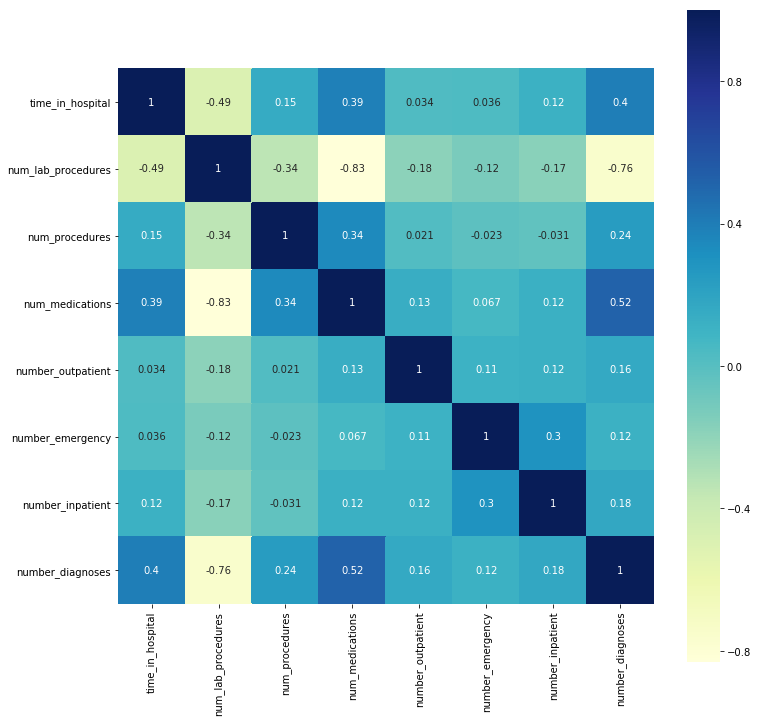
\includegraphics[scale = 0.45]{numfeatscorr} $$ 
Correlation amongst continuous features was computed using the correlation formula. It was found that there was heavy dependency between number of lab procedures and number of diagnoses. This would make sense considering diagnoses are made after doing some laboratory testing. In addition, there is moderate correlation between number of medications and number of lab procedures. The number of lab procedures and number of emergency visits were two of the least correlated features when compared to the other continuous features. 

\section{Preprocessing}
\subsection{Imputation of Missing Values}
After analyzing the data, it is time to pre process the data so it is ready for the model creation. The first step is to impute missing values. \\
Figure 4a: $$ 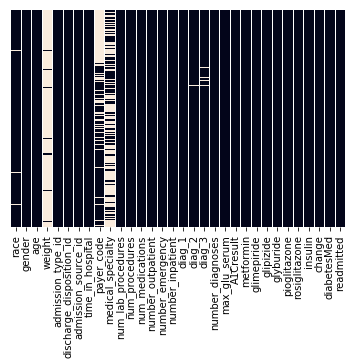
\includegraphics[width=\textwidth]{missingval} $$ 
According to this heat map, the columns ``weight,", ``payer code" and ``medical specialty"  have heavy amount of missing data. In fact, the weight feature is missing values in $96\%$ of its records which the other two features having missing value in $\approx 40\%$ and $\approx 50\%$ of the record respectively. In addition, the ``race" feature and all three diagnoses features have little missing value. To handle this, drop the ``weight" feature since it nearly has no data at all. For the remaining missing value features, use a random forest classifier, with $5$ trees, to find the missing values. This is done by separating the dataset by records that don't have the missing feature, call it training data, and records that have the missing data, testing data. The class label of this classifier will be the feature with missing value. Using a random forest is best here because as an ensemble classifier, it performs implicit feature selection to use the best features to split into branches and reduce the variance of the estimator as more and more trees are used. Therefore a separate random forest classifier is run for each missing value feature. 

\subsection{Feature Selection}
Before wondering if the class label is evenly balanced, appropriate features must be selected first so that it does not affect the SMOTE oversampling algorithm afterwards. Feature selection will be run on the dataset with missing values imputed using random forest. The features will be selected by choosing the top $33\%$ that is related to the class label via a $\chi^2$ test. In a $\chi^2$ test (for independence), the null hypothesis is that the feature and the class label are independence whereas the alternative hypothesis is that the feature and the class label are not independent. The feature selector will pick the top $33\%$ of features that have an association with the class label. To begin with, the dataset has $186$ dummified/numerical features which will then be reduced to $62$. After the features are selected, it will be joined with the class labels for further preprocessing.

\subsection{Imbalanced Issue} 
The next step in preprocessing the data is checking the distribution of class labels. \\
Figure 4b: $$ 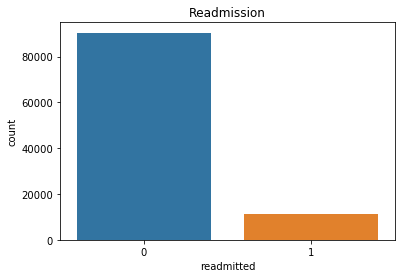
\includegraphics[scale = 0.6]{readmissioncount} $$ 
According to this bar graph, there is nearly $8$ times more records of people not being readmitted than people who are readmitted. This dataset is imbalanced. To tackle this issue, the SMOTE algorithm will be used to oversample from the smaller class label observations so that the number of class label equals the number of class label for non-readmission. In the SMOTE algorithm, a ratio, $r$, between the number of majority examples and number of minority examples is first calculated. Then for each minority example, its $k$ nearest minority neighbors (where $k \geq r -1$) are found and $r-1$ neighbors are randomly selected. From this, synthetic samples are randomly generated along the lines joining the minority sample and its $r-1$ selected neighbors. 

\section{Model}
\subsection{Individual Algorithms} 
There are five classification algorithms that will be used, of which three to go to each ensemble model. The five algorithms are: 
\begin{itemize} \item Perceptron \item Naive Bayes Classifier \item Decision Tree \item Linear Support Vector Classifier \item Extra Tree Classifier \end{itemize} 
In the perceptron algorithm, a hyperplane is attempted to be created that separates two class labels. It does this by instantiating a zero vector and computing $\hat{y_i}$ for each data point, where $\hat{y}_i = \text{sign}(w^Tx_i)$. For each $\hat{y}_i$ calculated, if $y_i \neq \hat{y}_i$, then $w$ is incremented by $\alpha(y_ix_i)$ where $\alpha$ is a learning rate. This is continued for all $y$ values. The final $w$ is then used to classify new data. This algorithm is easy to implement and only uses informative points. However if the data is not linearly separable, the algorithm will not converge. In addition, it can only learn linear functions and can overfit the data. \\~\\
In the Naive Bayes classifier algorithm, the probability of attaining each class label, $P(y_i)$ by itself is first calculated. Then for each attribute value $x_j$ of each attribute, its posterior probability, $P(x_j ~|~ y_i)$ is estimated. Then to find the class label of a new observation, it would be whichever value of $y_i$ that gives the highest posterior probability $$ y^* = \text{argmax}_{y_i \in Y} \left( P(y_i) \prod_{x_j^* \in X^*} P(x_j^* ~|~ y_i) \right) $$ 
This is based upon Bayes Rule for Posterior Probability: 
$$ P(Y_v ~|~ X_i = u_1, \dots, X_n = u_n) = \frac{P(X_1 = u_1,\dots,X_m = u_n ~|~ Y=v)P(Y=v)}{P(X_1=u_1,\dots,X_m=u_m)} $$ 
The Naive Bayes algorithm will be configured with the Gaussian distribution. This can be done since the dataset is large and by the Central Limit Theorem, the distribution of the dataset is normally distributed and has a mean $\mu$ and standard deviation $\sigma$.\\~\\
In the decision tree classifier algorithm , a tree is constructed from the top down by finding the purest subtree that give the greatest information gain. The algorithm will run as it is with one tree only. This is a step back from a random forest which utilizes multiple trees to do bagging and create an ensemble model. \\~\\
In the linear support vector classifier algorithm, data is separated by a hyperplane $w^Tx + b = 0$ where values above the plane are classified as one class and values below the plane are classified as the other plane. It does this by minimizing $ \frac{1}{2}w^Tw$ while also subject to $y_i(w^Tx_i + b) \geq 1$ for all $i = 1,2,\dots,N$. Once the hyperplane is found, new data can be classified with respect to the hyperplane position. In this project, the classifier will use the ``linear" parameter to have more flexibility in the choice of penalties and loss function. This is helpful because it helps doing classification on a large dataset.  Using a simple support vector classifier will not scale well if there is a large number of observations. \\~\\
In the extra tree classifier algorithm, an ensemble of randomized trees are created. It does so without bagging. Each tree is built from the original learning sample. At each test node, the best split is made among $K$ random splits. These splits are determined by random selection of features without replacement and a threshold. It comes close to being a random forest classifier except there is more randomization which hinders the idea that the best splits will be found. In this project, $3$ randomized trees will be constructed for each run of extra tree and a prediction will be made based on the majority vote of the three randomized trees. \\~\\
A model will be created using each of these five classification algorithms. 

\subsection{Ensemble Models}
Three forms of ensemble models were created for analysis in this project. The first form consists of three of the five algorithms as listed below. In each of these ensemble models, a voting classifier will fit the data to each of the classifier and make a prediction from it. Then a majority vote is taken among the three predictions for each of the new observation. The ten combinations of algorithms are shown below: 
\begin{itemize} 
\item Perceptron, Naive Bayes, Decision Tree
\item Perceptron, Naive Bayes, Linear SVC 
\item  Perceptron, Naive Bayes, Extra Tree 
\item  Perceptron, Decision Tree, Linear SVC 
\item Perceptron, Decision Tree, Extra Tree 
\item Perceptron, Linear SVC, Extra Tree 
\item Naive Bayes, Decision Tree, Linear SVC
\item Naive Bayes, Decision Tree, Extra Tree
\item Naive Bayes, Linear SVC, Extra Tree
\item Decision Tree, Linear SVC, Extra Tree \end{itemize} 
The second from of ensemble model that will be created is an ensemble of all five of these classification algorithms. \\~\\
The third form of ensemble model that will also be created is a good ol' fashioned random forest. This is a widely used ensemble model that is simple and easy to implement without many hyper-parameters. It produces amazing results for both classification and regression problems and in record time as well. One could just use a random forest to make ensemble models. But where's the creativity in that? Hence this project will create this model last to compare how other algorithms and ensembles did relative to the random forest classifier. In addition, no hyper-parameters will be modified so as to improve its accuracy. 

\section{Results}
For each model, a confusion matrix is created to show the number of true positives, true negatives, false positives and false negatives calculated. It is presented in a heat map where a color of yellow indicates low counts and a color of blue indicates high counts. In addition, a table of metrics is also provided showcasing the accuracy, precision, recall, and F1 score of each model and the time it took to create and evaluate it. \\~\\
Classifier Model: Perceptron
$$ 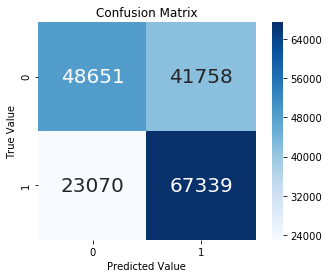
\includegraphics[scale = 0.5]{perceptron} ~~~~ \scoring{0.64}{0.61}{0.74}{0.67}{1.25} $$ 

Classifier Model: Naive Bayes 
$$ 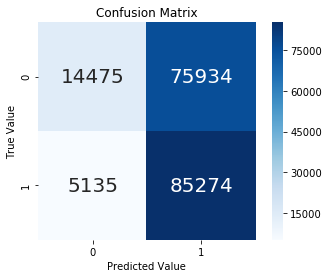
\includegraphics[scale = 0.5]{naivebayes} ~~~~ \scoring{0.55}{0.52}{0.94}{0.67}{1.00} $$ 

Classifier Model: Decision Tree
$$ 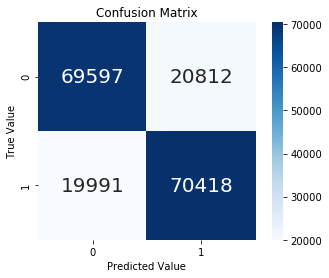
\includegraphics[scale = 0.5]{decisiontree} ~~~~ \scoring{0.77}{0.77}{0.77}{0.77}{8.58} $$

Classifier Model: Linear SVC
$$ 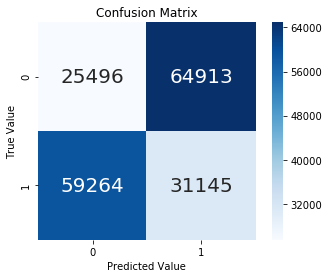
\includegraphics[scale = 0.5]{svc} ~~~~ \scoring{0.31}{0.32}{0.34}{0.33}{6.57} $$

Classifier Model: Extra Tree 
$$ 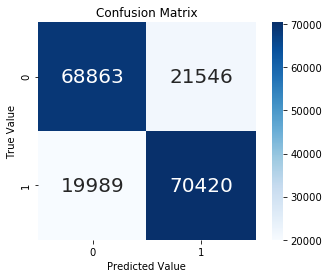
\includegraphics[scale = 0.5]{extratree} ~~~~ \scoring{0.77}{0.76}{0.77}{0.77}{2.04} $$

Ensemble Model: Perceptron, Naive Bayes, Decision Tree
$$ 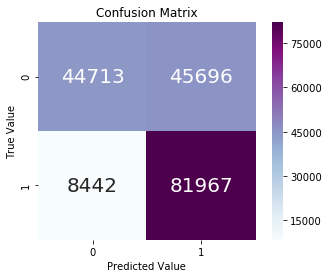
\includegraphics[scale = 0.5]{P:NB:DT} ~~~~ \scoring{0.70}{0.64}{0.90}{0.75}{11.30} $$ 

Ensemble Model: Perceptron, Naive Bayes, Linear SVC
$$ 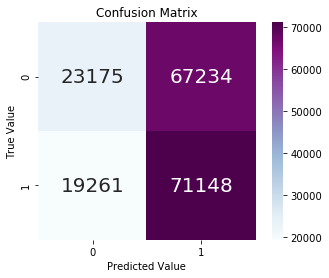
\includegraphics[scale = 0.5]{P:NB:SVC} ~~~~ \scoring{0.52}{0.51}{0.78}{0.62}{9.10} $$
 
Ensemble Model: Perceptron, Naive Bayes, Extra Tree
$$ 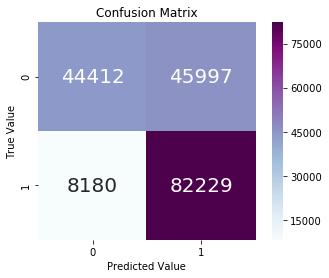
\includegraphics[scale = 0.5]{P:NB:ET} ~~~~ \scoring{0.70}{0.64}{0.90}{0.75}{4.45} $$

Ensemble Model: Perceptron, Decision Tree, Linear SVC 
$$ 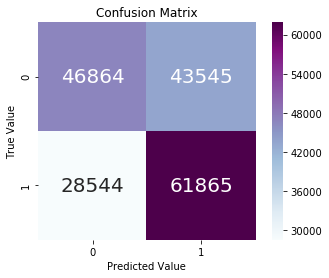
\includegraphics[scale = 0.5]{P:DT:SVC} ~~~~ \scoring{0.60}{0.58}{0.68}{0.63}{17.51} $$

Ensemble Model: Perceptron, Decision Tree, Extra Tree
$$ 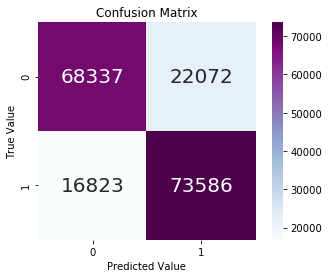
\includegraphics[scale = 0.5]{P:DT:ET} ~~~~ \scoring{0.78}{0.76}{0.81}{0.79}{12.66} $$

Ensemble Model: Perceptron, Linear SVC, Extra Tree
$$ 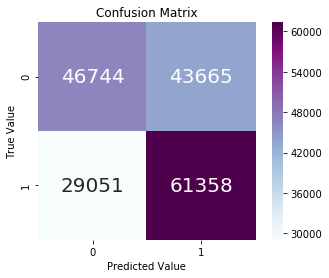
\includegraphics[scale = 0.5]{P:SVC:ET} ~~~~ \scoring{0.59}{0.58}{0.67}{0.62}{9.86} $$

Ensemble Model: Naive Bayes, Decision Tree, Linear SVC 
$$ 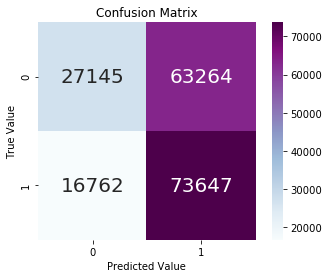
\includegraphics[scale = 0.5]{NB:DT:SVC} ~~~~ \scoring{0.55}{0.53}{0.81}{0.64}{18.16} $$

Ensemble Model: Naive Bayes, Decision Tree, Extra Tree
$$ 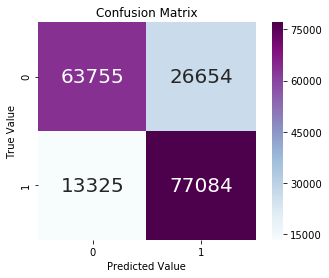
\includegraphics[scale = 0.5]{NB:DT:ET} ~~~~ \scoring{0.77}{0.74}{0.85}{0.79}{12.00} $$

Ensemble Model: Naive Bayes, Linear SVC, Extra Tree
$$ 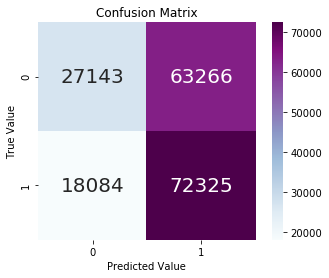
\includegraphics[scale = 0.5]{NB:SVC:ET} ~~~~ \scoring{0.55}{0.53}{0.79}{0.64}{9.44} $$

Ensemble Model: Decision Tree, Linear SVC, Extra Tree 
$$ 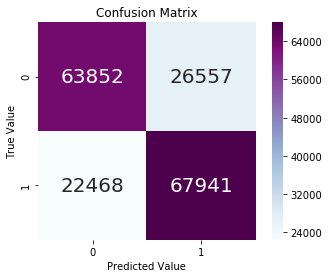
\includegraphics[scale = 0.5]{DT:SVC:ET} ~~~~ \scoring{0.72}{0.71}{0.75}{0.73}{16.69} $$

Ensemble Model: Perceptron, Naive Bayes, Decision Tree, Linear SVC, Extra Tree
$$ 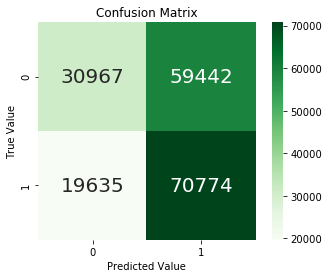
\includegraphics[scale = 0.5]{All5Classifiers} ~~~~ \scoring{0.56}{0.54}{0.78}{0.64}{18.24} $$

Ensemble Model: Random Forest
$$ 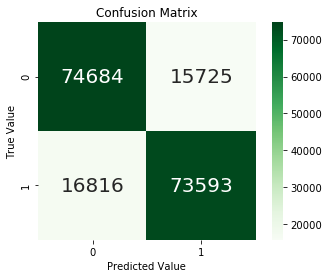
\includegraphics[scale = 0.5]{RandomForest} ~~~~ \scoring{0.82}{0.82}{0.81}{0.81}{9.72} $$

A graph is created to show the accuracies of all the models. 
$$ 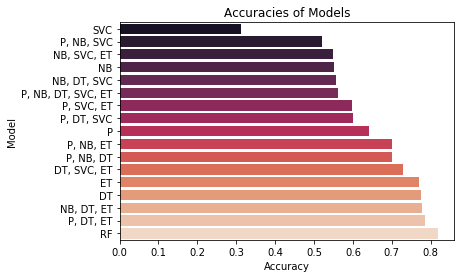
\includegraphics[scale = 0.7]{accuracy} $$ 
A graph is created to show the F1 score of all the models. 
$$ 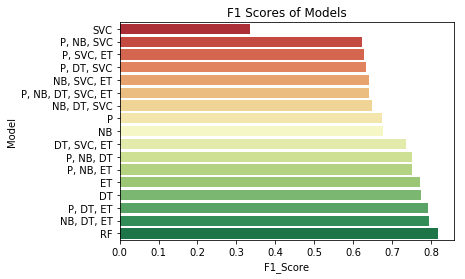
\includegraphics[scale = 0.7]{f1score} $$ 
A graph is created to show the time efficiency of all the models. 
$$ 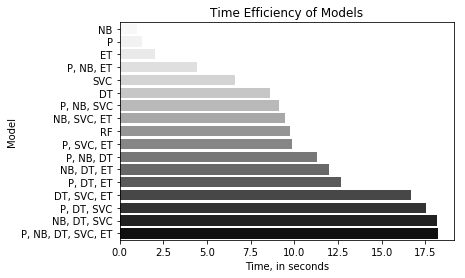
\includegraphics[scale = 0.7]{runtime} $$ 

\newpage
\section{Conclusion} 
A multitude of simple and ensemble models were created to predict readmission of diabetic patients. But only a few gave satisfying results. When looking at the accuracy of the models, the support vector classifier algorithm performed the worse, at $31\%$, which the random forest algorithm performed the best, at $82\%$. Coming at a close second and third place is the ensemble model of perceptron, decision tree and extra tree as well as the ensemble model of Naive Bayes, decision tree and extra tree. Looking at the accuracies in general, it appears that if trees are used in any of the models, it will improve the overall accuracy of the model. In fact, just using a single decision tree or extra tree gave an overall accuracy of $77\%$. Also worth noting is that when an ensemble was created from all five classifiers, it performed slightly worse than if a tree model was excluded from the ensemble. This is interesting because both the SVC and Naive Bayes classifiers did not perform well on its own and yet it does better together with a tree than an ensemble of all $5$ classifiers. \\~\\
The F1 score was another statistic used to understand how well each model did. It is the harmonic mean of the precision and recall. $$ \text{F1} = \left( \frac{ \text{recall}^{-1} + \text{precision}^{-1}}{2}\right)^{-1} =  2 \cdot \frac{\text{precision} \cdot \text{recall}}{\text{precision} + \text{recall}} $$ 
Similar analysis was found when evaluating on basis of the F1 score of all the models. The SVC model performed the worse, at $33\%$. The next worst model was the ensemble of perceptron, Naive Bayes and SVC which has a F1 score of more than $60\%$. The best F1 score was achieved by the random forest classier at more than $80\%$. The next best model was the ensemble of Naive Bayes, decision tree and extra tree at an F1 score of $79\%$. It is also seen that any form of trees, whether singular, randomized or bagged, did fairly well on it own as well as in the ensemble models. In addition, the perceptron algorithm did decent on it own, just behind models with trees. Just like with accuracy, the ensemble model of all five classifier also had a low F1 score. \\~\\
Just for fun, the time it took to create and evaluate each model was also taken note of. It should be of no surprise that the ensemble of all five classifiers took the greatest amount of time to execute. The models that took the least time to be made and tested were the Naive Bayes classifier, perceptron classifier and extra tree classifier, in that order. Then it should be of no surprise that the ensemble model that took the least time to be created and tested was the one of those three classifiers. The models that performed well in terms of accuracy and F1 score had moderate timing as compared to other models, not too time consuming but also not quick as a flash. Note that all models were constructed and tested in under $20$ seconds. Despite all this, the time efficiency should not be taken into consideration for how well the model did. 

The best model that can be used to predict readmission for diabetic patients is the random forest classifier.

\newpage
\section{Appendix A: Data Visualizations of Categorical Features}
Figure A1: 
 $$ 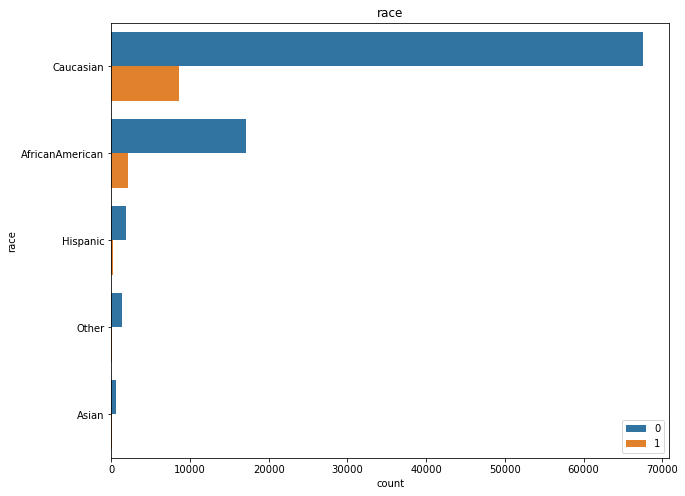
\includegraphics[scale = 0.35]{race}$$ 
It is clear that the Caucasian race makes up most of the dataset, followed by African Americans. In addition, looking at the people who were readmitted within $30$ days, most were either Caucasian or African American. The number of people who were readmitted and were Hispanic, Asian or other fell to less than $1,000$. 
\\~\\
Figure A2: $$ 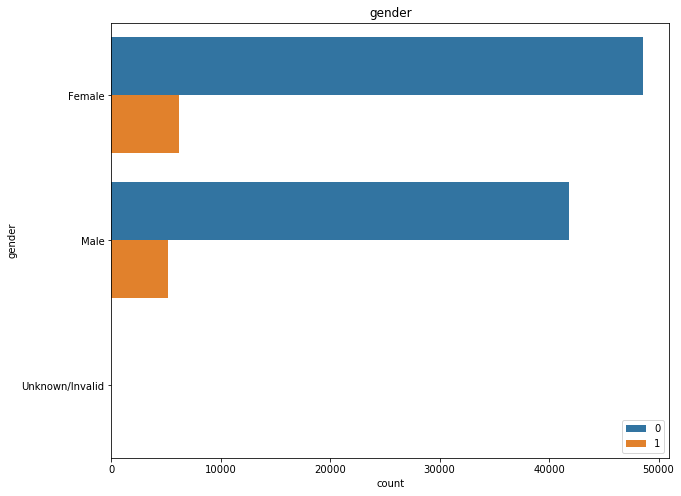
\includegraphics[scale = 0.35]{gender}$$ 
For male patients, the number of people who were readmitted was roughly $\frac{1}{8}$ of the number of men who were not readmitted. For female patients, the number of people who were readmitted was roughly $\frac{1}{10}$ of the number of women who were not readmitted. 

Figure A3: $$ 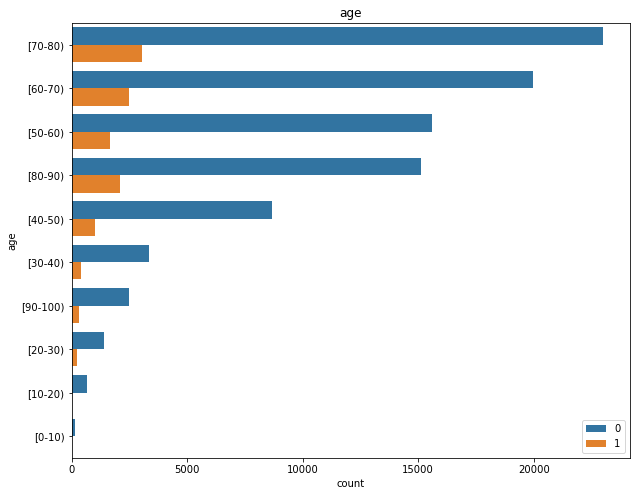
\includegraphics[scale = 0.35]{age}$$ 
As age increased, more and more people were readmitted within $30$ days. As for non-readmission, The age group of 70 to 80 had the most number of people who were not readmitted despite it also having the second highest number of readmission. 
\\~\\
Figure A5: $$ 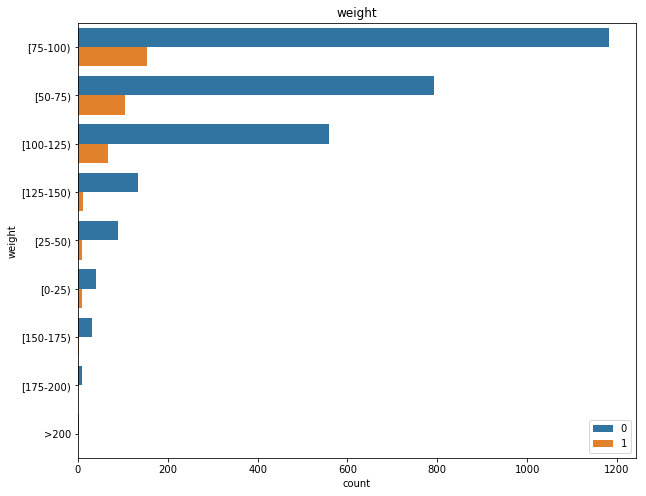
\includegraphics[scale = 0.35]{weight}$$ 
The weight groups of $50$ to $75$ and $75$ to $100$ were the most occurring weights. for both readmission and non-readmission. 

Figure A6: $$ 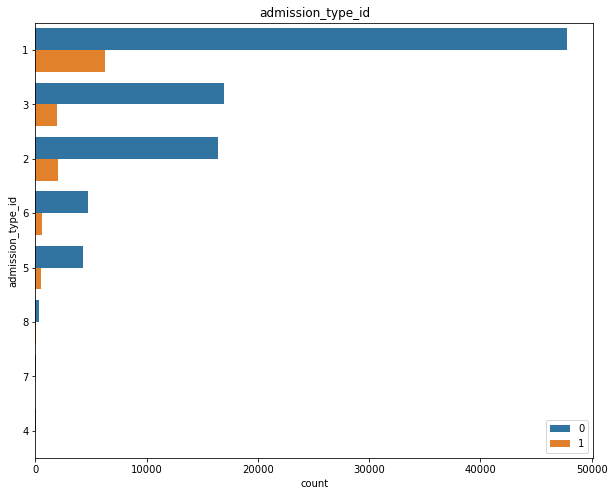
\includegraphics[scale = 0.35]{admission_type_id}$$ 
Most of the admission types for readmission and non-readmission belong to patients who had the ID $1$, $3$ or $2$. Which admission type it is specifically is not provided but it can be from emergency, urgent, elective, newborn and not available. 
\\~\\
Figure A7:  $$ 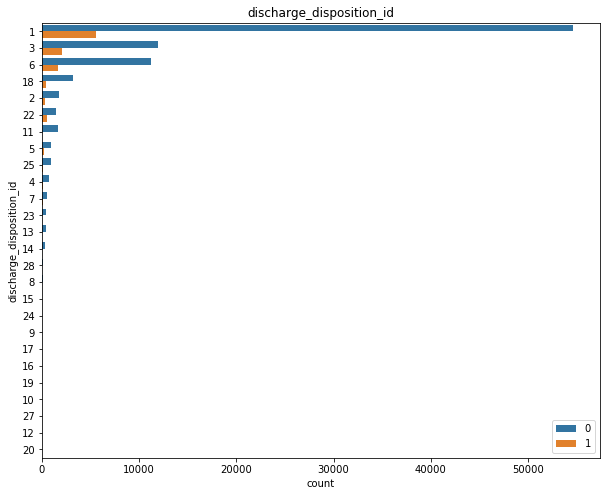
\includegraphics[scale = 0.35]{discharge_disposition_id}$$ 
Most of the discharge disposition ID values were $1$, $3$, and $6$. Exact reference is not found but it could be from discharged to home, expired and not available. 

Figure A8: $$ 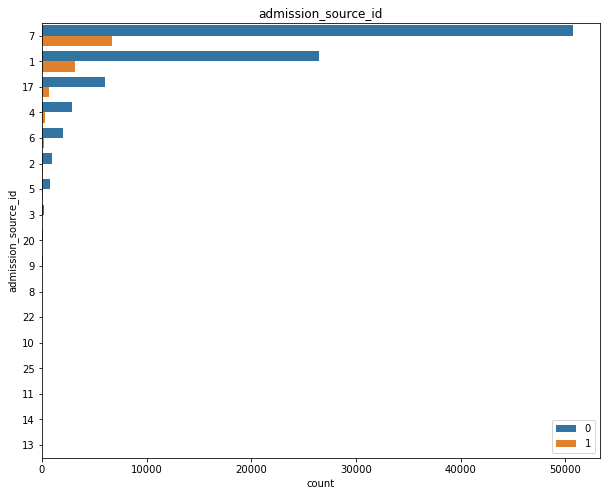
\includegraphics[scale = 0.35]{admission_source_id}$$ 
Most of the admission source ID values were $1$ and $7$. 
\\~\\
Figure A9: $$ 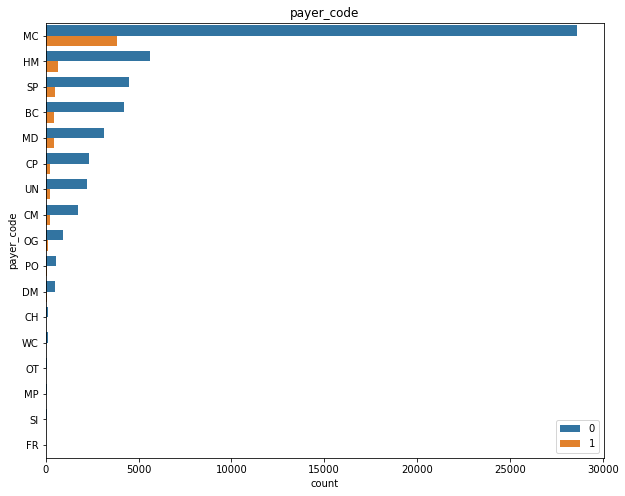
\includegraphics[scale = 0.35]{payer_code}$$ 
For both readmission and non-readmission, the most frequent payer code used was MC and HM. This is most likely an insurance plan such as Medicare or self-pay. 


Figure A10: $$ 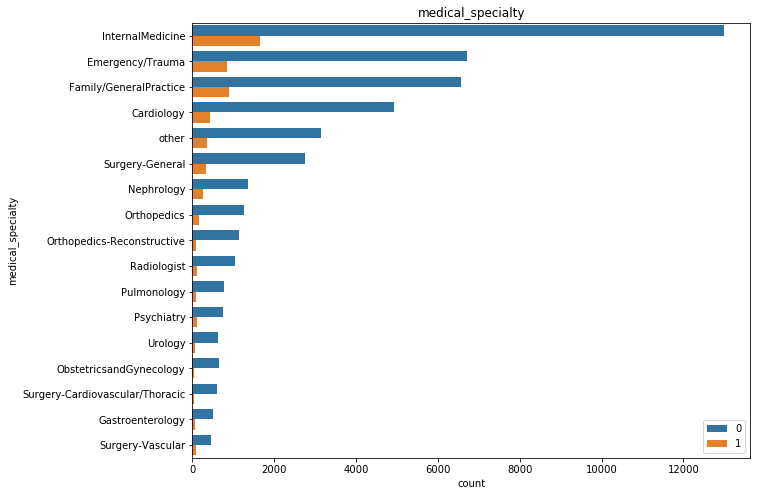
\includegraphics[scale = 0.35]{medical_specialty}$$ 
The specialties of the doctors associated with these patients range from internal medicine, emergency/trauma, family/general practice and cardiology.  
\\~\\
Figure A11: $$ 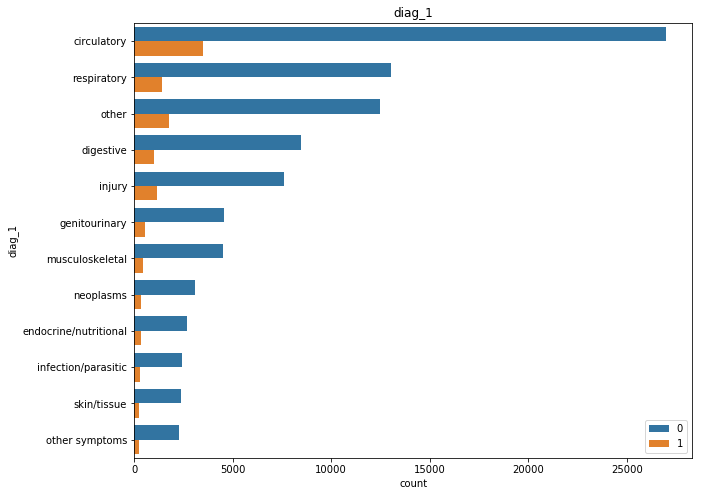
\includegraphics[scale = 0.35]{diag_1}$$ 
There is some connection between the medical specialties and the primary diagnoses. Most frequent diagnoses related to the circulatory system or the respiratory system. Both of these systems are closely monitored by the specialties given above. The ``other" specialty is also frequent meaning a variety of other uncommon diagnoses were given as well. 

Figure A12: $$ 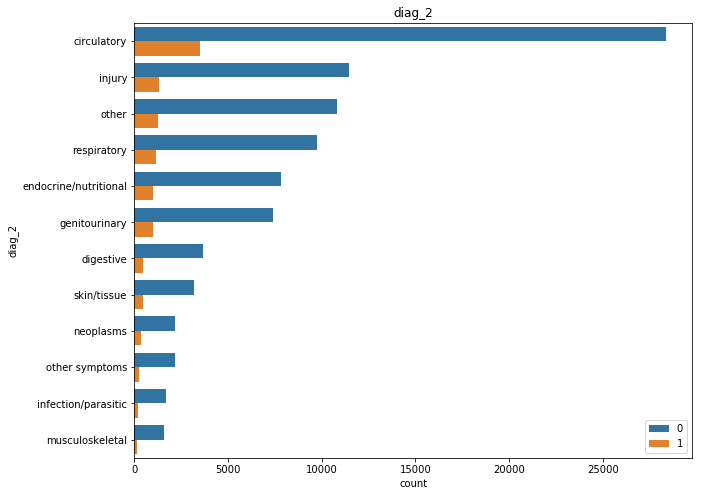
\includegraphics[scale = 0.35]{diag_2}$$ 
Figure A13: $$ 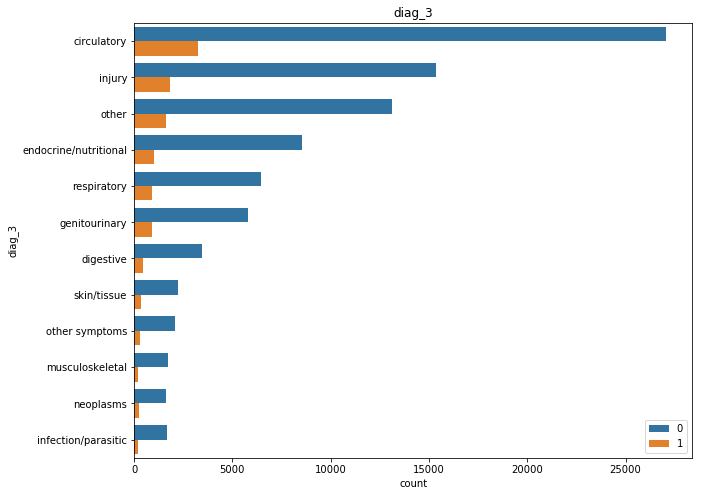
\includegraphics[scale = 0.35]{diag_3}$$
For both the secondary diagnoses and the second secondary diagnoses, most frequent ones given out were circulatory, injury, ``other," respiratory or endocrine/nutritional. 
\\~\\
Figure A14: $$ 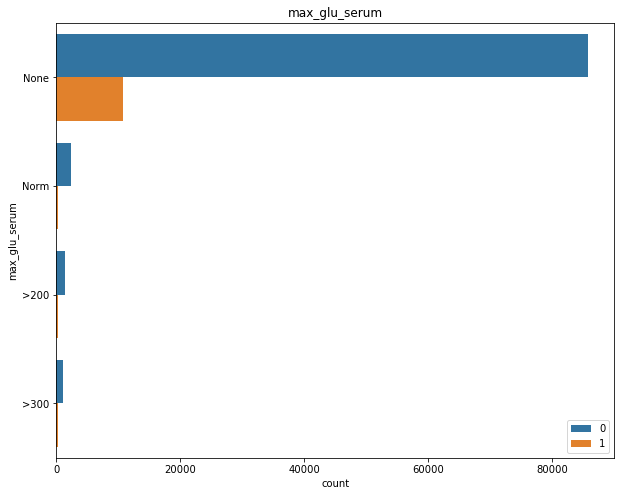
\includegraphics[scale = 0.35]{max_glu_serum}$$ 
A big majority of the patient who were readmitted did not have their glucose serum test taken. 

Figure A15: $$ 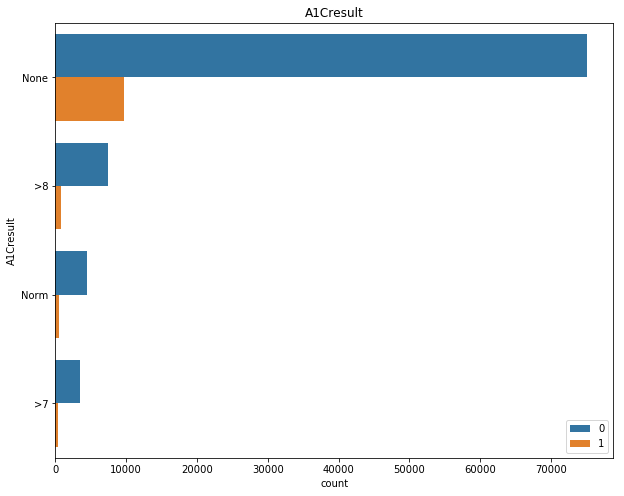
\includegraphics[scale = 0.35]{A1Cresult}$$ 
Patients who were readmitted did not have an A1c test result. For the few that do, their test result indicates greater than $8\%$. 
\\~\\
Figure A16: $$ 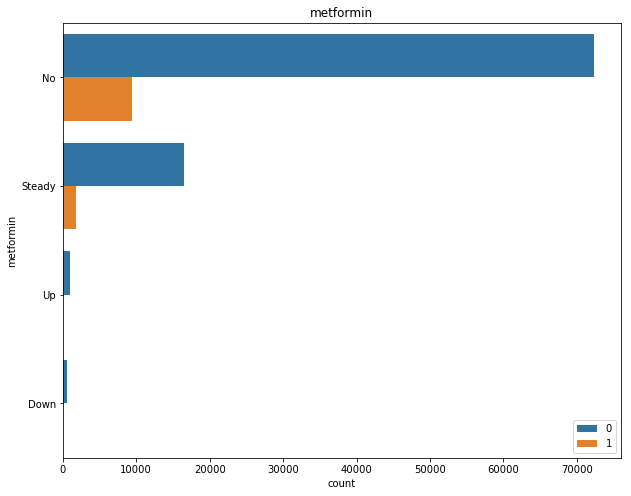
\includegraphics[scale = 0.35]{metformin}$$ 
Figure A17: $$ 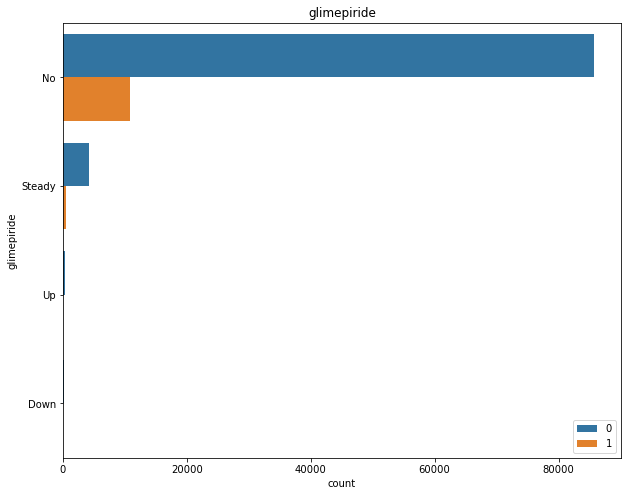
\includegraphics[scale = 0.35]{glimepiride}$$ 
Figure A18: $$ 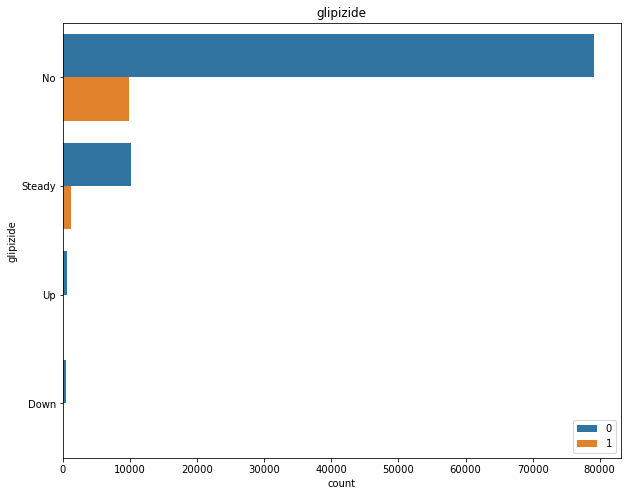
\includegraphics[scale = 0.35]{glipizide}$$ 
Figure A19: $$ 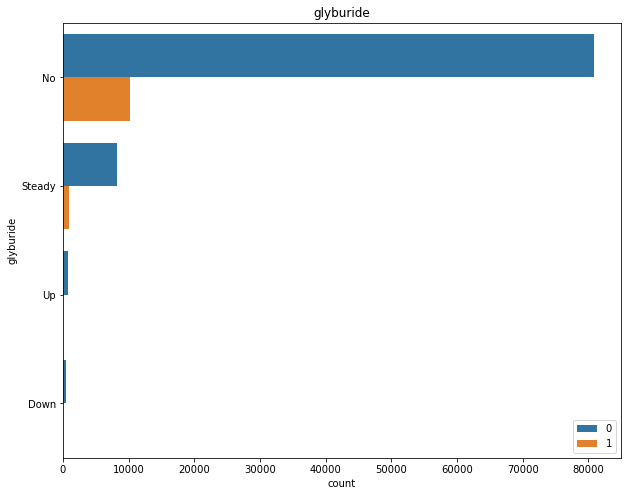
\includegraphics[scale = 0.35]{glyburide}$$ 
Figure A20: $$ 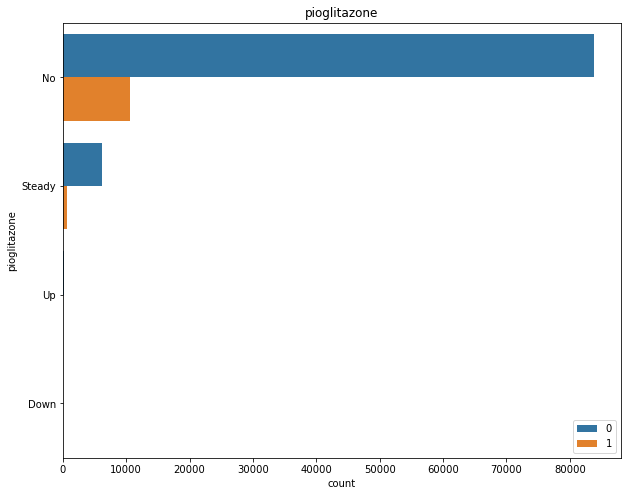
\includegraphics[scale = 0.35]{pioglitazone}$$ 
Figure A21: $$ 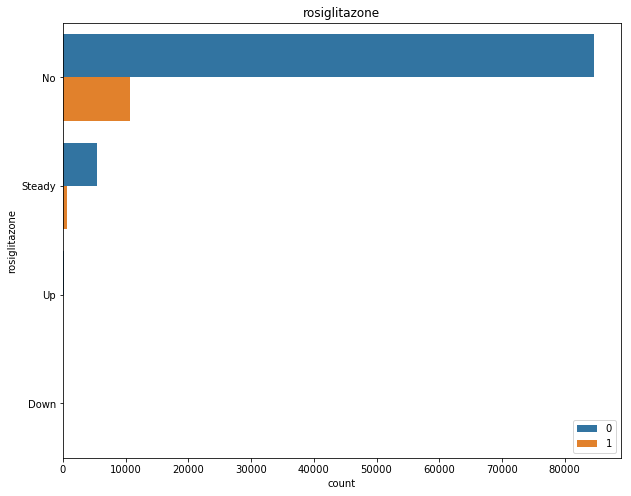
\includegraphics[scale = 0.35]{rosiglitazone}$$ 
Patients who were readmitted either had no prescription for 
\begin{multicols}{3} \begin{itemize}
\item metformin \item glimepiride \item glipizide \item glyburide \item pioglitazone \item rosiglitazone \end{itemize} \end{multicols} or were on a steady dose. 

Figure A22: $$ 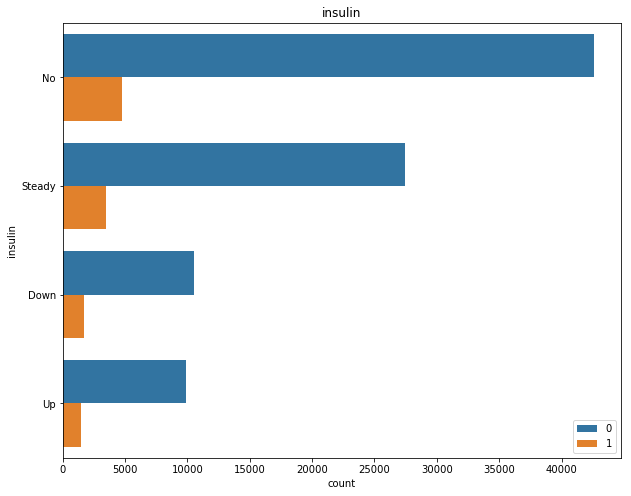
\includegraphics[scale = 0.35]{insulin}$$ 
Insulin dosage were more uniformly distributed than the previous medications. Most patients who were readmitted either had no prescription for insulin or were on a steady dose. It is worth noting that that are at least a thousand people who have either gone up or down on their insulin dosage. 
\\~\\
Figure A23: $$ 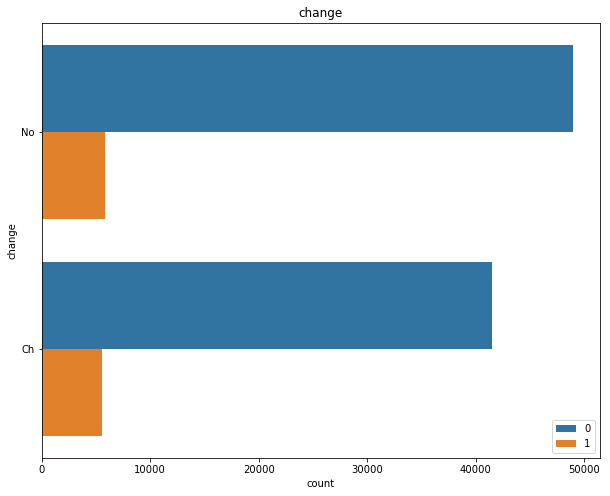
\includegraphics[scale = 0.35]{change}$$ 
The fact that if a change was done do not differ for the patients who were readmitted or not readmitted. Equal number of readmitted patients had their medication changed or not changed. 
\newpage
\section{Appendix B: Data Visualizations of Continuous Features}
The numerical features' distribution, after normalization, was now graphed with the distinction being made with the class label of readmission. \\
Figure B1: $$ 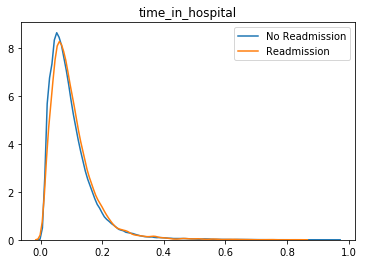
\includegraphics[scale = 0.45]{time_in_hospital}$$ 
The distribution for both readmitted patients and non-readmitted patients and their time in hospital is skewed right where a majority of the values lie between $0.0$ and $0.4$. \\~\\
Figure B2: $$ 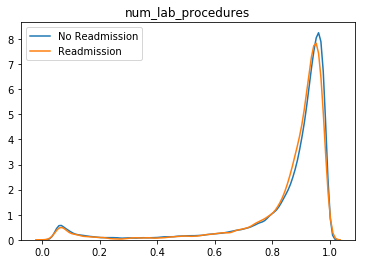
\includegraphics[scale = 0.45]{num_lab_procedures}$$ 
The distribution for both readmitted patients and non-readmitted patients and their number of lab procedures is skewed left with a majority of values between $0.6$ and $1.0$, with a slight number of values at $0.1$. \newpage
Figure B3: $$ 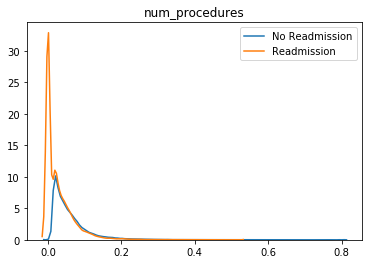
\includegraphics[scale = 0.45]{num_procedures}$$ 
The distribution for readmitted patients and number of non-lab procedures is more extremely skewed right than that for the non-readmitted patients. Despite this. most values lie between $0.0$ and $0.2$. \\~\\
Figure B4: $$ 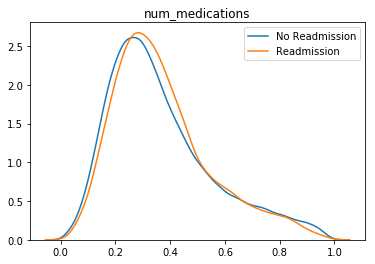
\includegraphics[scale = 0.45]{num_medications}$$ 
The distribution for number of medications for both readmitted and non-readmitted patients are similar. Both are uniformly distributed with a slight skew to the right. All values lie between $0.0$ and $1.0$ \\~\\
Figure B5: $$ 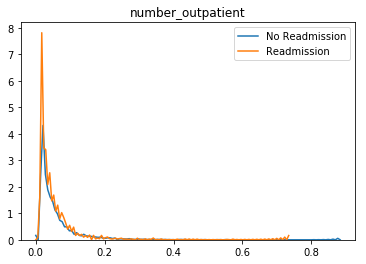
\includegraphics[scale = 0.45]{number_outpatient}$$ 
The distribution of number of outpatient with readmitted patients is more extreme than for the non-readmitted patients. Both distributions are heavily skewed right and have most density within $0.0$ and $0.2$. \\~\\
Figure B6: $$ \includegraphics[scale = 0.45]{number_emergency}$$ 
The distribution of number of emergency normalized for both readmitted and non-readmitted patients were skewed right with most density lying in between $0.0$ and $0.2$. \\~\\
Figure B7: $$ \includegraphics[scale = 0.45]{number_inpatient}$$ 
The distribution of number of inpatient for readmitted patients was more extreme than for the non-readmitted patients while also being skewed right. Most values lied between $0.0$ and $0.1$. \\~\\
Figure B8: $$ \includegraphics[scale = 0.45]{number_diagnoses}$$ 
The number of diagnoses for both readmitted patients and non-readmitted patients were uniformly distribution with a slightly longer tail on the right. All values lied between $0.0$ and $0.8$. 

\end{document} 